\documentclass[a4paper]{IEEEconf}

\usepackage{csquotes}
\usepackage[dutch]{babel}
\usepackage[backend=biber,style=ieee,natbib=true]{biblatex}
\addbibresource{references.bib}
\usepackage{url}
\usepackage{hyperref}
\usepackage{graphicx}

\newcommand{\citeGartner}{\cite{Gartner:08Q2, Gartner:08Q3, Gartner:08Q4, Gartner:10Q1, Gartner:10Q2, Gartner:10Q3, Gartner:10Q4, Gartner:11Q1, Gartner:11Q2, Gartner:11Q3, Gartner:11Q4, Gartner:12Q1, Gartner:12Q2, Gartner:12Q3, Gartner:12Q4, Gartner:13Q1}}
\newcommand{\citeGartnerTab}{\cite{Gartner:11tab,Gartner:12tab}}
\renewcommand{\vec}[1]{\mathbf{#1}}
\newcommand{\html}[1]{{\small \texttt{#1}}}
\newcommand{\lsfrac}[2]{{\large $\sfrac{#1}{#2}$}}
\newcommand{\tick}{\checkmark}

\begin{document}
\title{Een vergelijkende studie van cross-platform tools voor het ontwikkelen van mobiele applicaties}
\author{
    Michiel~Staessen \\
    \begin{affiliation}
       Departement computerwetenschappen\\
       KU~Leuven\\
    \end{affiliation} \\
    \email{michiel.staessen@student.kuleuven.be}
}
\maketitle

\begin{abstract}
    % Abstract should be 150 words or less.
    Het ontwikkelen van mobiele applicaties voor meerdere platformen is een tijdrovende en dure bezigheid. Omwille van deze reden zoeken meer en meer bedrijven hun toevlucht in cross-platform tools (CPT's) voor het ontwikkelen van mobiele applicaties (of apps). In opdracht van Capgemini, een internationaal consultingbedrijf, presenteert dit artikel een methode voor het evalueren en selecteren van cross-platform tools in een bedrijfsomgeving. Aansluitend worden de resultaten gepresenteerd van de toepassing van deze methode op de native SDK's en twee cross-platform tools, Apache Cordova of PhoneGap en Motorola Rhodes. De tools worden getest op hun inzetbaarheid voor het maken van smartphone en tablet applicaties voor Android en iOS.
\end{abstract}

\section{Inleiding}

Smartphones zijn razend populair en de verkoop ervan is op zijn minst indrukwekkend: sinds 2009 hebben de fabrikanten een samengestelde jaarlijkse groei van 57,61\% weten te realiseren, uitgaande van wereldwijd marktonderzoek door Gartner \citeGartner. Deze groei wordt voornamelijk aangedreven door goedkope Android toestellen die de plaats innemen van de traditionele GSM. 

Een soortgelijk scenario speelt zich af op de markt van de tablets. Volgens een schatting van IDC zullen tablet fabrikanten tussen 2012 en 2016 wereldwijd een samengestelde jaarlijkse groei van 23,3\% realiseren \cite{IDC:tablet}.

De huidige smartphonemarkt wordt gedomineerd door het Apple/Google duopolie. Van de 700 miljoen verkochte smartphones is 85\% een Android toestel of iPhone. Door netwerkeffecten is het erg moeilijk voor andere platformen om marktaandeel te verkrijgen. Desalniettemin blijven ontwikkelaars naar alternatieven zoeken omdat ze als de dood zijn voor vendor lock-in \cite{VMDE:2013}.

Cross-platform tools (CPT's) laten ontwikkelaars toe om applicaties te ontwikkelen voor meerdere platformen tegelijk, vertrekkende van een (quasi) identieke codebase. CPT's verlagen daarmee zowel toetredings- als uittredingsdrempels (``lock-in''). Door een CPT te gebruiken, krijgt de ontwikkelaar eenvoudig toegang tot nieuwe platformen en kan de ontwikkelaar gemakkelijker naar een ander platform migreren \cite{VMCPT:2012}.

CPT's proberen een oplossing te bieden voor drie problemen \cite{VMCPT:2012}:

\begin{itemize}
    \item Het eerste doel is uiteraard het overwinnen van platform fragmentatie want de apparaten zijn op zeer diverse vlakken erg verschillend: besturingssysteem, versie van het besturingssysteem, schermgrootte, schermresolutie, processorkracht, \ldots 
    \item Daarnaast vereenvoudigen CPT's ook de toegang tot nieuwe platformen en schermen. Hoewel op dit ogenblik CPT's voornamelijk gebruikt worden voor het ontwikkelen van smartphone en tablet applicaties, kunnen CPT's ook gebruikt worden voor het ontwikkelen van applicaties voor desktops, TV's en andere media.
    \item Tot slot kan het gebruik van CPT's leiden tot een effici\"enter beheer van ontwikkelingsmiddelen. Een applicatie voor meerdere platformen ontwikkelen impliceert namelijk dat (vaak verschillende) teams meerdere codebases en functionaliteit moeten synchroniseren over de verschillende platformen. Dit is een tijdrovende en dure bezigheid.
\end{itemize}

\section{Mobiele architecturen}

Er zijn tot op heden vijf architecturen gekend om applicaties (of apps) op meerdere platformen beschikbaar te maken: native apps, mobile web apps, hybrid apps, interpreted apps en cross-compiled apps \cite{Friese}.

\subsection{Native apps}

Native apps zijn de de facto architectuur voor het ontwikkelen van een mobiele applicatie en vormen dus de baseline voor de vergelijking van de architecturen. 

Native apps worden ontwikkeld met de SDK die aangeleverd wordt door de ontwikkelaar van het platform. Voor Android worden native applicaties geschreven in Java, voor iOS worden deze applicaties geschreven in Objective-C. Daarenboven hebben native apps een uiterlijk dat consistent is met het uiterlijk van het besturingssysteem (ook native look \& feel genoemd) en kunnen ze het volledige potentieel van het toestel benutten waardoor ze het meest performant zijn. 

\subsection{Mobile web apps}

Mobile web apps zijn mobiele websites en worden geopend in de web browser van het mobiele toestel. Omdat elk platform over een browser beschikt en omdat de HTML-specificatie platform onafhankelijk is, zijn mobiele web apps de meest eenvoudige manier om voor meerdere platformen te ontwikkelen. Er zijn echter ook nadelen verbonden aan mobiele web apps.

Mobiele web apps worden verspreid met behulp van een URL en kunnen dus niet gevonden worden in applicatiewinkels, zoals de App Store en Google Play. Hoewel de HTML5 specificatie een zekere toegang verleent tot het apparaat, kunnen niet alle functies van het mobiele apparaat aangesproken worden. Bovendien is de ondersteuning van dergelijke API's vaak gebrekkig in mobiele browsers \cite{MobileHTML5}. Ook de performantie laat vaak te wensen over.

Omdat de mobiele web app in de browser draait, kan deze ook geen gebruik maken van native UI elementen en kan deze dus ook geen native look \& feel aanbieden. Of dit een nadeel is, staat nog ter discussie. Websites voldoen aan de ``one size fits all'' filosofie en mogen als dusdanig een eigen look \& feel hebben \cite{Mahemoff:2011}.

Cross-Platform Tools voor web app ontwikkeling zijn HTML5 frameworks waaronder jQuery Mobile, Sencha Touch, KendoUI, Zepto.js, en DHTMLX Touch.

\subsection{Hybrid apps}

Hybrid apps zijn de combinatie van native apps en mobiele web apps. De mobile website wordt verpakt in een native omhulsel en dit omhulsel kan extra functionaliteit openstellen naar de applicatie indien de browser bepaalde functionaliteit mist. De communicatie tussen de applicatie en het omhulsel verloopt via een JavaScript bridge. Op deze manier kunnen hybrid apps vooralsnog het volledige potentieel van het mobiele apparaat benutten.

Voor de eindgebruiker is er weinig verschil tussen een hybrid apps en native apps omdat deze apps via de gewoonlijke kanalen te verkrijgen zijn (applicatiewinkels). Hybrid apps hebben geen native uiterlijk omdat ze doorgaans geen native UI elementen kunnen gebruiken voor de user interface. Hybrid apps zijn sterk afhankelijk van de browser en dus laat ook de performantie van hybrid apps vaak te wensen over. 

Ondanks de nadelen, zijn hybrid apps toch interessant en in het bijzonder voor web ontwikkelaars die de overstap maken naar mobiele applicaties. Zij kunnen op deze manier hun kennis van webtechnologie gebruiken om mobiele applicaties te maken. Omdat de applicatie zelf in HTML geschreven is, laat dit toe om updates te verspreiden zonder tussenkomst van de applicatiewinkel en ondersteunen CPT's voor hybrid apps doorgaans meer platformen.

Cross-Platform Tools die dit patroon volgen zijn onder meer Apache Cordova, Sencha Cmd, Trigger.io en Kony

\subsection{Interpreted apps}

Interpreted apps maken gebruik van een tussenliggende taal die wordt vertaald in native instructies at runtime. Dit is min of meer vergelijkbaar met de Java VM die Java bytecode omzet in machinecode. Deze architectuur vereist uiteraard wel dat de runtime-omgeving meegeleverd wordt met de applicatie. Hierdoor neemt de applicatie meer ruimte in beslag op het apparaat.

De performantie van interpreted apps is sterk afhankelijk van de gebruikte tussentaal en vertaler maar is doorgaans beter dan web of hybrid apps. Omdat de interpreted apps vertaald worden naar platformspecifieke code, kunnen ze wel gebruik maken van native UI elementen en zullen ze de native look \& feel kunnen aanbieden. Interpreted apps kunnen verspreid worden via app stores omdat ze --- net als hybride apps --- verpakt worden als native apps. 
 
Cross-platform tools die deze architectuur omarmen zijn onder andere Appcelerator Titanium en Rhodes.

\subsection{Cross-compiled apps}

Cross-compiled apps maken --- net zoals interpreted apps --- gebruik van een tussenliggende taal. Alleen worden de instructies in deze taal niet tijdens het uitvoeren maar tijdens het compileren vertaald. Bijgevolg hoeft er geen runtime meegeleverd te worden met de applicatie.

De performantie is afhankelijk van de gebruikte cross-compiler maar doorgaans gelijkaardig aan de performantie van native apps. Ook de native UI elementen kunnen gebruikt worden waardoor de applicatie een vertrouwd uiterlijk heeft.

Xamarin and MoSync zijn cross-platform tools die deze architectuur gebruiken.

\section{Methodologie}

De methodologie die gebruikt wordt in dit onderzoek is gebaseerd op een generische software selectie methode, voorgesteld door \citet{Jadhav:2011}. Deze methode bestaat uit zes aanpasbare stappen die in de volgende alinea's besproken worden.

\subsection{Definieer selectiecriteria}

In de eerste stap worden de selectiecriteria bepaald. Deze criteria zijn de functionele en non-functionele vereisten waaraan een CPT moet voldoen om in aanmerking te komen voor verdere evaluatie. Omdat dit onderzoek wordt gevoerd in opdracht van consultingbedrijf Capgemini, ligt de focus op applicaties voor de bedrijfswereld. De selectiecriteria werden bepaald op de startvergadering en houden in dat:

\begin{itemize}
    \item de CPT applicaties kan maken voor zowel Android als iOS,
    \item de CPT applicaties kan maken voor zowel smartphones als tablets,
    \item de CPT bruikbaar is voor het maken van business applicaties,
    \item de CPT een geschikte maturiteit heeft,
    \item de CPT een goede ondersteuning heeft door de ontwikkelaar of de gemeenschap.
\end{itemize}

\subsection{Identificeer mogelijke kandidaten}

In de deze stap wordt gezocht naar mogelijke, bruikbare kandidaten. Tijdens deze zoektocht worden de selectiecriteria nog niet in rekening gebracht. Deze fase is namelijk louter een ontdekkingsfase. Tijdens het onderzoek werden 160 mogelijke tools ge\"identificeerd uit een in 2012 voltooide studie van VisionMobile \cite{VMCPT:2012} en een nog onvoltooide studie van  research2guidance \cite{Research2guidance}. 

\subsection{Selecteer kandidaten voor evaluatie}

In de derde stap worden de selectiecriteria uit de eerste stap gebruikt om de lijst van kandidaten, verkregen in de tweede stap, te filteren. Uit de lijst van overgebleven tools, werd voorrang verleend aan 7 tools omdat deze ofwel erg populair zijn of specifiek ingezet worden voor het ontwikkelen van applicaties in de bedrijfswereld. Uit deze 7 tools werden twee tools geselecteerd, namelijk Apache Cordova en Motorola Rhodes. Cordova werd geselecteerd voor haar populariteit, Rhodes omwille van zijn bedrijfscontext.

\subsection{Definieer evaluatiecriteria}

Tijdens deze stap worden de criteria waarop de alternatieven beoordeeld worden, vastgelegd. Hiervoor werd gekeken naar de literatuur \cite{Gartner:CPT:2011, VMCPT:2012} en er werden interviews afgenomen bij een ontwikkelaar, een architect en een verkoper van Capgemini. Er zijn 11 evaluatiecriteria geformuleerd en deze zijn georganiseerd in een boomstructuur met drie hoog-niveau categorie\"en om de vergelijking eenvoudiger te maken. De literatuur suggereert namelijk dat mensen slechts in staat zijn om rekening te houden met $7 \pm 2$ stukken informatie \cite{Miller:1956}. De evaluatiecriteria zijn:

\begin{itemize}
    \item \textbf{Portabiliteit} meet het vermogen van een tool om bepaalde facetten van de software of het ontwikkelingsproces te hergebruiken voor de verschillende platformen.
    \begin{itemize}
        \item \textbf{Platformondersteuning} meet het aantal ondersteunde platformen, naast Android en iOS. 
        \item \textbf{Hergebruik van tools} meet in hoeverre het mogelijk is om de ontwikkelomgeving te hergebruiken.
        \item \textbf{Hergebruik van code} meet hoeveel code van een applicatie hergebruikt kan worden tussen platformen onderling.
    \end{itemize}
    \item \textbf{Gebruikerservaring van de applicatie} gaat na in hoeverre een cross-platform applicatie kan tippen aan een native applicatie.
    \begin{itemize}
        \item \textbf{Integratie met het platform} test de mogelijkheid om een applicatie te integreren met het platform.
        \begin{itemize}
            \item \textbf{Toegang tot de hardware} gaat op zoek naar de mogelijkheden tot integratie met de hardware. 
            \item \textbf{Integratie met platform-specifieke diensten} gaat op zoek naar integratiemogelijkeden met services zoals push-notificaties.
        \end{itemize}
        \item \textbf{Gebruikersinterface} onderzoekt de mogelijkheden van de grafische gebruikersinterface.
        \begin{itemize}
            \item \textbf{Native look \& feel} gaat na of de tool gebruik kan maken van de native gebruikersinterface elementen.
            \item \textbf{Gebruikersinterface elementen} bestudeerd de mogelijkheid om een rijke gebruikersinterface aan te bieden met de elementen die voorhanden zijn.
        \end{itemize}
        \item \textbf{Performantie} beschrijft de snelheid waarmee de applicatie reageert op invoer.
    \end{itemize}
    \item \textbf{Productiviteit} beschrijft de effici\"entie bij het maken van applicaties bij het gebruik van een zekere tool. 
    \begin{itemize}
        \item \textbf{Hergebruik van vaardigheden} kijkt naar de mogelijkheden om reeds verworven vaardigheden te hergebruiken.
        \item \textbf{Gereedschap} focust op de kwaliteit van het aangeboden gereedschap om de applicatie te maken.
        \item \textbf{Testen} onderzoekt de mogelijkheden van de tool om geautomatiseerde testen te schrijven. 
    \end{itemize}
\end{itemize}

Merk op dat deze criteria geen kosten bevatten. De kosten en baten zijn met opzet van elkaar gescheiden gehouden zodat op het einde van de vergelijking een aparte kosten-batenanalyse kan worden gemaakt.

\subsection{Evalueer de alternatieven}

Met de evaluatiecriteria uit de vorige stap, kunnen de alternatieven nu ge\"evalueerd worden. \citet{Jadhav:2011} dwingen geen specifieke techniek af voor deze evaluatie maar laten de keuze over aan de onderzoeker. Voor dit onderzoek werd gekozen voor het analytisch hi\"erarchisch proces (AHP), ontworpen door Thomas L. Saaty \cite{Saaty:1980, Saaty:1990}. Deze methode berekent, op basis van het eigenwaardenprobleem, gewichten of scores voor zowel evaluatiecriteria en alternatieven. Deze gewichten zijn afkomstig uit paarsgewijze vergelijkingen waarbij gebruik gemaakt kan worden van zowel kwalitatieve als kwantitatieve evaluatiecriteria. Bovendien geeft de methode een indicatie van de hoeveelheid inconsistentie die aanwezig is in het gegeven oordeel. Naast het feit dat deze methode meermaals succesvol is toegepast in de literatuur, zijn dit de voornaamste redenen voor het selecteren van deze methode. 

In de eerste fase worden de evaluatiecriteria gewogen. In de tweede fase worden alle alternatieven aan een vergelijking onderworpen en worden voor elk criterium gewichten toegekend aan de alternatieven. In de laatste fase worden all gewichten gecombineerd door de som te berekenen van het product van een gewicht voor een bepaald alternatief met betrekking tot een bepaald criterium en het gewicht van dat criterium (additieve weging). De alternatieven kunnen dan gerangschikt worden op basis van de grootte van hun totaalgewicht.

\subsection{Selecteer het beste alternatief}

In de laatste stap, wordt het beste alternatief gekozen. De tool die het hoogste scoort in de evaluatie is daarbij niet noodzakelijk ook het beste alternatief. Bij het kiezen van het beste alternatief dienen de voordelen en de kosten tegenover elkaar afgewogen worden want geen enkel bedrijf zal haar middelen verspelen aan een ineffici\"ente tool. De kosten worden in dit onderzoek voorgesteld door de tijd die nodig is om de applicatie te ontwikkelen. Een applicatie bestaat namelijk uit een aantal lijnen code die in een bepaalde tijd moeten geschreven worden door een aantal mensen die moeten betaald worden.

\section{Geselecteerde cross-platform tools}

\subsection{Apache Cordova}

Apache Cordova\footnote{\url{http://cordova.apache.org}}, beter gekend als PhoneGap, is een open-source CPT die toelaat hybride applicaties te ontwikkelen voor Android, iOS, Blackberry, WebOS, Windows 8, Windows Phone, Symbian, Tizen en Bada.

De tool maakt gebruik van HTML5, JavaScript en CSS voor de ontwikkeling van applicaties. Met behulp van een JavaScript bridge kan de applicatie toegang krijgen tot het platform. Alle device API's zijn beschikbaar in de vorm van plug-ins. Ontwikkelaars kunnen ook hun eigen plug-ins maken indien ze specifieke native code op het platform willen aanroepen vanuit de HTML5 applicatie.

Cordova heeft een Apache 2.0 licentie en wordt beheerd door de Apache Software Foundation. PhoneGap is een distributie van Cordova, geleverd door Adobe \cite{LeRoux:2012}. Adobe biedt ook een clouddienst aan voor het compileren van PhoneGap applicaties. 

\subsection{Motorola Rhodes}

Motorola Rhodes\footnote{\url{http://docs.rhomobile.com/rhodes/introduction}} is eveneens een open-source CPT die toelaat interpreted/hybride applicaties te maken voor Android, iOS, BlackBerry, Windows Mobile en Windows Phone 8. 

De runtime omgeving van Rhodes is een Ruby-gebaseerd MVC framework voor web applicaties. De applicatie is dus een website (vergelijkbaar met Cordova) die op een lokale Ruby server op het apparaat zelf draait. 

Rhodes wordt ontwikkeld door Motorola Solutions en is vrij beschikbaar onder de MIT licentie. Een online dienst voor het compileren van Rhodes projecten is eveneens beschikbaar.

\section{Evaluatie}

Zoals gezegd worden eerst de criteria gewogen. Dit is gebeurd door de meningen over het relatieve belang van de criteria aan een ontwikkelaar en architect te vragen in de vorm van een enqu\^ete. Deze meningen werden met behulp van de AHP methode omgezet in gewichten. De verdeling van de gewichten wordt gevisualiseerd in Figuur \ref{fig:criteria_radar}. 

\begin{figure}[h!]
    \centering
    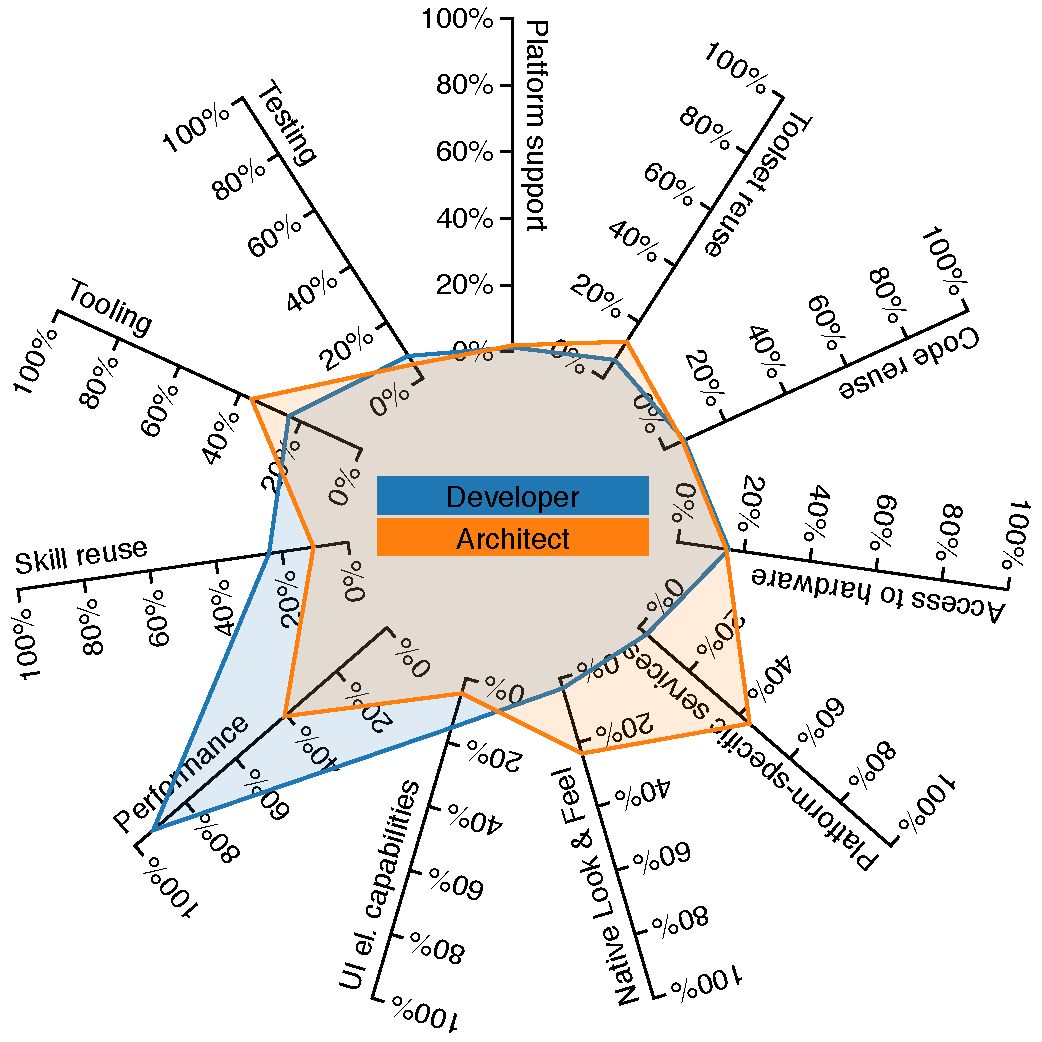
\includegraphics[width=0.45\textwidth]{../resources/figs/criteria_radar.pdf}
    \caption{Overzicht van de gewichtsverdeling van de evaluatiecriteria voor de ontwikkelaar en architect.}
    \label{fig:criteria_radar}
\end{figure}

Voor het vergelijken van de alternatieven (de tweede fase) wordt deels gebruik gemaakt van de beschikbare documentatie en deels gebruik gemaakt van ervaring die verworven werd tijdens het ontwikkelen van een proof-of-concept applicatie met elk van de tools. Deze ervaring is nodig om een waarheidsgetrouw oordeel te kunnen vellen over de inzetbaarheid van de tools in een bedrijfsomgeving en de proof-of-concept applicatie combineert een aantal elementen die typisch voorkomen in applicaties voor deze markt. De gewichten van de alternatieven worden gevisualiseerd in Figuur \ref{fig:alternatives_radar}.

\begin{figure}[h!]
    \centering
    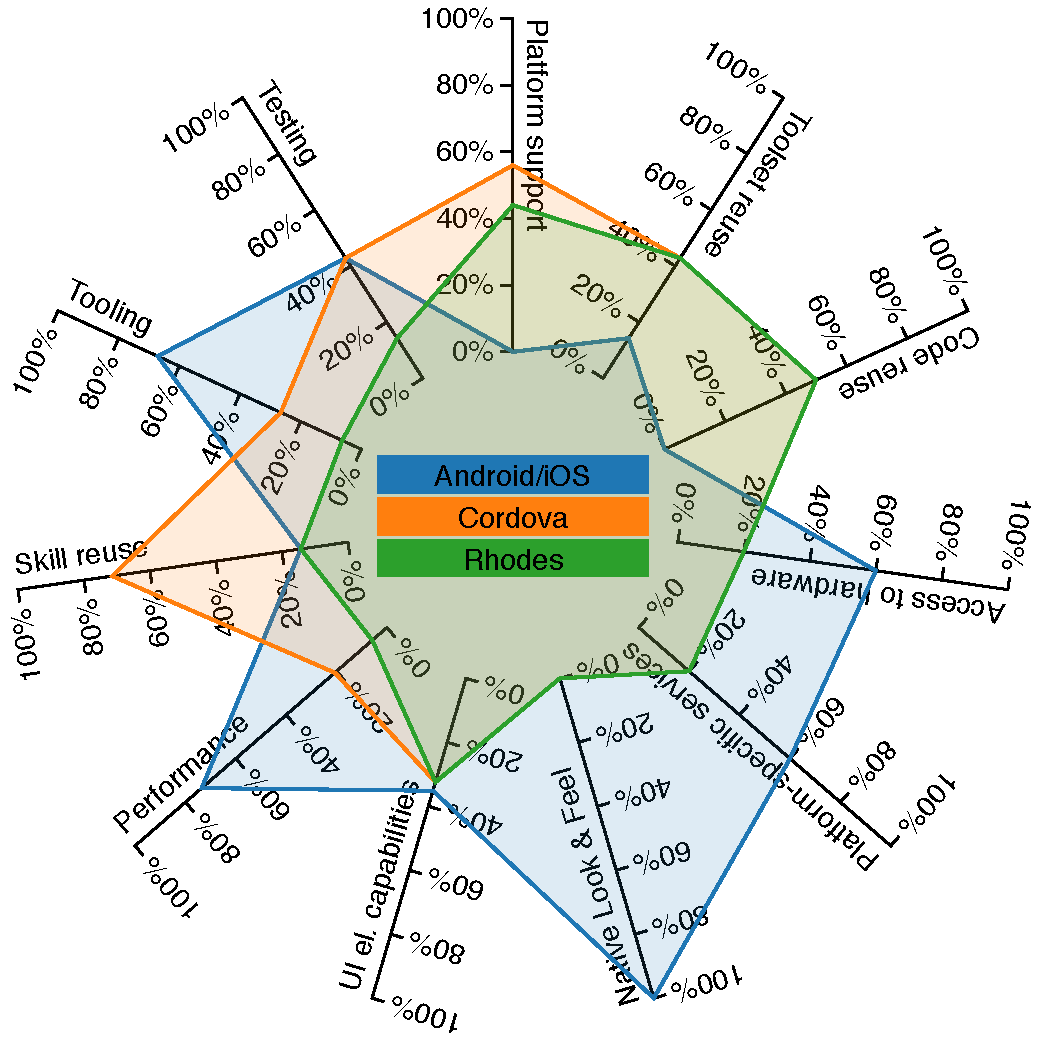
\includegraphics[width=0.45\textwidth]{../resources/figs/priority_radar.pdf}
    \caption{Overzicht van de gewichtsverdeling bij de alternatieven.}
    \label{fig:alternatives_radar}
\end{figure}

Vervolgens worden deze scores gecombineerd. De totaalgewichten worden weergegeven in Tabel \ref{tab:summary}. Omdat de meningen uiteenlopend zijn, wordt de evaluatie afzonderlijk uitgevoerd vanuit deze twee perspectieven. Uit de resultaten blijkt echter dat de rangschikking voor beide profielen dezelfde is en dus zal de volgorde eveneens behouden blijven bij het berekenen van het gemiddelde.

\begin{table}[h!]
    \centering
    \begin{tabular}{lccc}
        \hline
                     & Android/iOS & Cordova   & Rhodes    \\
        \hline
        Architect    & $59.99\%$   & $25.25\%$ & $14.75\%$ \\           
        Ontwikkelaar & $55.82\%$   & $30.77\%$ & $13.40\%$ \\
        \hline
        Gemiddelde   & $57.90\%$   & $28.01\%$ & $14.08\%$ \\
        \hline
    \end{tabular}
    \caption{Overzicht van de totaalscores van de alternatieven.}
    \label{tab:summary}
\end{table}

Tot slot worden de kosten en baten vergeleken. Er wordt geschat dat voor het ontwikkelen van Cordova applicaties ongeveer de helft van de tijd nodig is, vergeleken met native applicaties voor Android en iOS. Dit is het gevolg van de mogelijkheid om 100\% van de applicatiecode te kunnen hergebruiken op Android en iOS. Er wordt tevens geschat dat het ontwikkelen van Rhodes applicaties iets langer duurt dan Cordova applicaties omdat er minder kant-en-klare componenten zijn die samen met Rhodes gebruikt kunnen worden. Deze bevindingen worden getoond in Figuur \ref{fig:cost-benefit}.

\begin{figure}[h!]
    \centering
    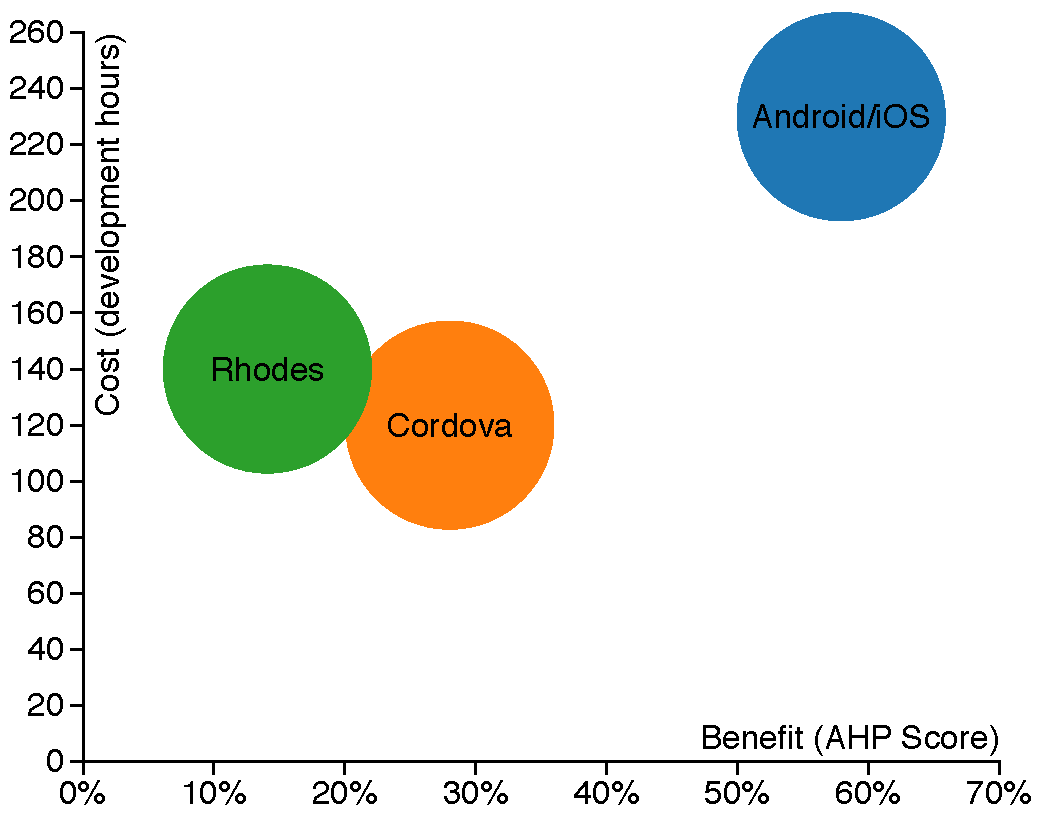
\includegraphics[width=0.45\textwidth]{../resources/figs/benefit-cost.pdf}
    \caption{Visualisatie van de kosten-batenanalyse.}
    \label{fig:cost-benefit}
\end{figure}

Uit deze figuur kan men concluderen dat Cordova en native Android/iOS een vergelijkbare kost-effectiviteit hebben. Voorlopig wordt het verlies in voordelen dus enkel gecompenseerd door een kortere projectduur. Indien echter binnenkort extra platformen (naast Android en iOS) ondersteund moeten worden, kan er drastisch op kosten bespaard worden door applicaties te ontwikkelen met Cordova op voorwaarde dat een zeker verlies van voordelen acceptabel is. 

\section{Gerelateerd werk}

De methode die in dit onderzoek gehanteerd wordt om cross-platform tools te evalueren en te selecteren is gebaseerd op literatuurstudies van \citet{Jadhav:2009}, \cite{Jadhav:2011}. Deze studies suggereren eveneens 3 methodes voor evaluatie waarvan het analytisch hi\"erarchisch proces van  \citet{Saaty:1980} gekozen werd.

Een andere bijdrage tot dit onderzoek is de studie van VisionMobile bij meer dan 2400 ontwikkelaars in 91 landen over het gebruik van cross-platform tools \cite{VMCPT:2012}. Deze studie onthult meerdere elementen die nuttig waren, zoals architecturen, alternatieven en redenen voor het selecteren of verlaten van bepaalde cross-platform tools.

\section{Besluit}

Dit artikel presenteert een methode voor het evalueren en selecteren van cross-platform tools voor gebruik in een bedrijfsomgeving en toont eveneens de resultaten na toepassing van deze methode op native Android en iOS en twee cross-platform tools, Apache Cordova en Motorola Rhodes. Het relatieve belang van de evaluatiecriteria werd vastgelegd door een ontwikkelaar en een architect bij Capgemini en dus geeft dit onderzoek geen algemeen beeld van de volledige industrie maar eerder een beeld voor het geval van CapGemini, indien de bevraagde personen representatief zijn voor Gapgemini in zijn geheel.

Het uiteindelijke resultaat van dit onderzoek is dat er momenteel nog weinig voordelen gehaald kunnen worden uit de beschouwde cross-platforms tools maar dit kan mogelijk veranderen in de toekomst, wanneer meer dan twee platformen ondersteund dienen te worden. Indien het verlies van voordelen acceptabel is, kan Cordova ervoor zorgen dat een hogere productiviteit en een lagere kost kan gerealiseerd worden.

\printbibliography
\end{document}